% Daftarche User Guide. Build with tools/build_docs.sh (XeLaTeX).
\documentclass[11pt]{article}
\usepackage{guide}
\input{version.tex}

\hypersetup{pdftitle={Daftarche User Guide}, pdfauthor={Vahid Anari},
  pdfsubject={User Guide for Daftarche \AppVersion}, pdfkeywords={Daftarche, bookkeeping, personal finance}}

\begin{document}

% ════════════════════════════════════════════════════════════════════════════
%  Cover
% ════════════════════════════════════════════════════════════════════════════
\thispagestyle{empty}
\AddToShipoutPictureBG*{%
  \put(0,0){\color{night}\rule{\paperwidth}{\paperheight}}%
  \put(0,\LenToUnit{\paperheight-0.5625\paperwidth}){
\includegraphics[width=\paperwidth]{../src/daftarche/data/icons/splash.png}}%
}
\begin{tikzpicture}[remember picture, overlay]
  \node[anchor=north west, inner sep=0pt] at ($(current page.north west)+(2.6cm,-2.6cm)$)
    {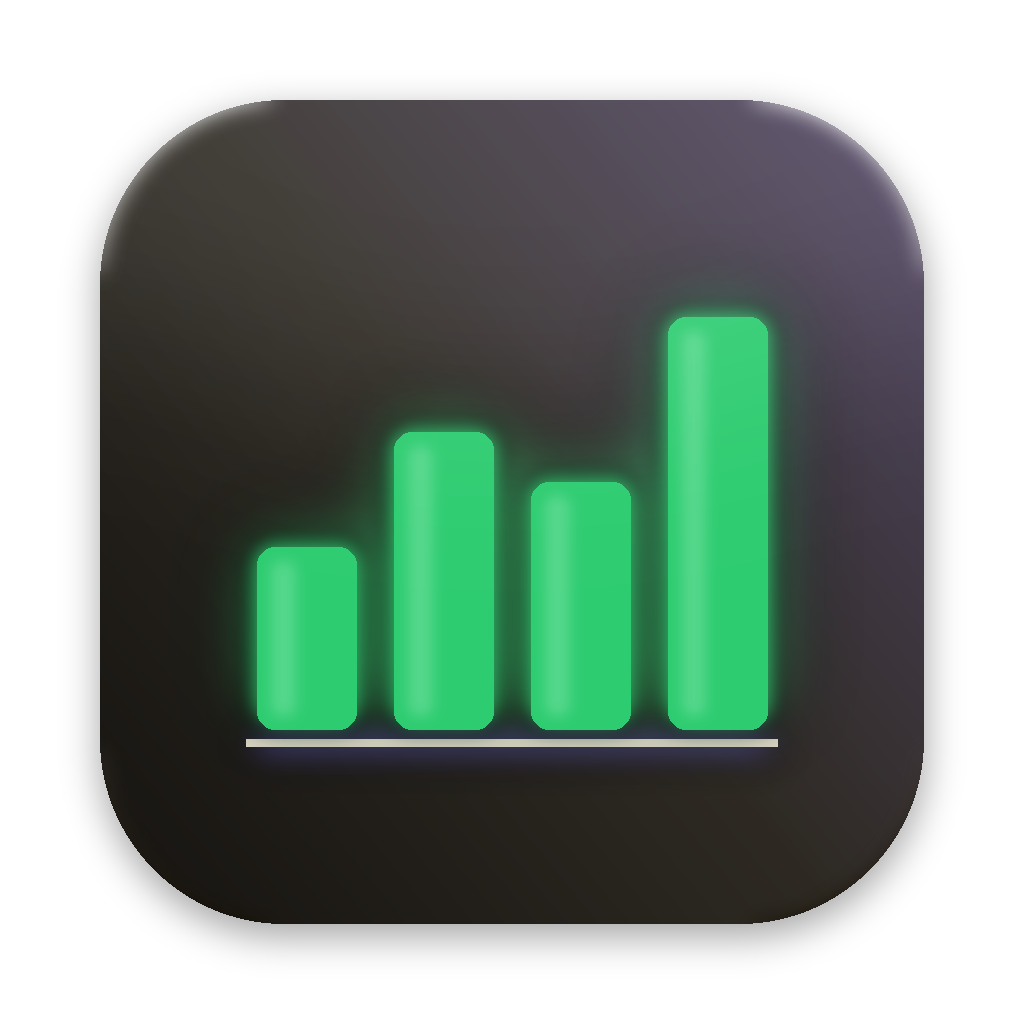
\includegraphics[width=2.4cm]{../src/daftarche/data/icons/app_icon.png}};
  \node[anchor=north west, text=white, font=\fontsize{54}{58}\selectfont\bfseries, inner sep=0pt]
    at ($(current page.north west)+(2.6cm,-5.6cm)$) {Daftarche};
  \node[anchor=north west, text=white!75!night, font=\LARGE, inner sep=0pt]
    at ($(current page.north west)+(2.7cm,-7.7cm)$) {Your own account book};
  \node[anchor=south west, text width=12.5cm, text=white!82!night, font=\large, inner sep=0pt, align=left]
    at ($(current page.south west)+(2.6cm,6.2cm)$)
    {\setstretch{1.3}See where your money goes. Daftarche reads the statements you download from
     your bank, sorts every purchase into categories, and shows it all in clear charts —
     privately, on your own computer.};
  \node[anchor=south west, fill=accent, text=white, rounded corners=8pt, inner xsep=12pt, inner ysep=7pt,
    font=\large\bfseries] at ($(current page.south west)+(2.6cm,3.2cm)$) {User Guide};
  \node[anchor=south west, text=white!60!night, font=\normalsize]
    at ($(current page.south west)+(6.4cm,3.42cm)$) {for version \AppVersion};
  \node[anchor=south west, text=white!78!night, font=\large, inner sep=0pt]
    at ($(current page.south west)+(2.6cm,1.9cm)$) {by Vahid Anari};
\end{tikzpicture}
\newpage

% ════════════════════════════════════════════════════════════════════════════
%  Contents
% ════════════════════════════════════════════════════════════════════════════
\thispagestyle{empty}
{\Huge\bfseries What's inside\par}
\vspace{0.4em}{\large\color{dim}Read the first three chapters to get going. The rest is there when you need it.\par}
\vspace{1.4em}
\newcommand{\tocline}[3]{%
  \begin{tcolorbox}[enhanced, colback=white, colframe=line, boxrule=0.5pt, arc=8pt, left=4pt, right=10pt,
    top=3pt, bottom=3pt, before skip=0pt, after skip=4pt, hyperref=ch:#1]
  \begin{tabular}{@{}m{1.3cm}@{}m{11.6cm}@{}m{1.2cm}@{}}
    \tikz\node[fill=accent, text=white, rounded corners=5pt, minimum size=0.85cm, font=\Large\bfseries]{#1};
    & {\large\bfseries #2}\par{\color{dim}#3}
    & \hfill{\color{dim}\pageref{ch:#1}}
  \end{tabular}\end{tcolorbox}}
\tocline{1}{Welcome}{What Daftarche does, and what it keeps private}
\tocline{2}{Getting started}{Install it, open it, and look around}
\tocline{3}{Bringing in your bank statements}{Download a statement, import it, and let Daftarche sort it}
\tocline{4}{Sorting your money}{Categories, shops, rules that learn, and the To Review list}
\tocline{5}{The four tabs}{Dashboard, Transactions, Charts and Accounts, one by one}
\tocline{6}{Moving money between your accounts}{Transfers, credit card payments and savings}
\tocline{7}{Special cases}{Refunds, one payment in several categories, money lent to friends}
\tocline{8}{Making it yours}{Your categories, accounts and tags; colours, font and theme}
\tocline{9}{Your data and backups}{Where everything is kept, and how to get it back}
\tocline{10}{Keeping Daftarche up to date}{New versions in one click}
\tocline{11}{Shortcuts and answers}{The keys worth knowing, and common questions}
\newpage

% ════════════════════════════════════════════════════════════════════════════
\chapter{Welcome}{What Daftarche does, and what it keeps private.}\label{ch:1}

\textbf{Daftarche} (Persian for \emph{“little account book”}) helps you see where your money goes.
You download your bank statements, Daftarche reads them, and every purchase, pay cheque and
transfer ends up in one place, sorted into categories you choose: groceries, rent, eating out,
salary, and so on. Then the charts show you, month by month, what came in and what went out.

\screenshot[0.92\linewidth]{dashboard.png}{The Dashboard: your accounts on the left, income and spending each month,
and where the money went. (All screenshots in this guide show invented data.)}

\subsection{Three kinds of money}
Everything in Daftarche is one of three kinds, and each has its own colour throughout the app:

\begin{inshort}
\begin{tabular}{@{}p{2.2cm}p{12.1cm}@{}}
\income   & Money that comes in: your salary, a refund from the government, a gift.\\[0.35em]
\expense  & Money you spend: groceries, rent, a coffee. A refund from a shop is a \emph{negative} expense,
            so it lowers what you spent in that category.\\[0.35em]
\transfer & Money that moves between your own accounts, such as paying off your credit card or
            putting money into savings. It is neither income nor spending.
\end{tabular}
\end{inshort}

\subsection{Your data stays with you}
Daftarche never connects to your bank and never sends your data anywhere. Everything is kept in
a single file on your own computer, and Daftarche makes a backup copy of it every time it starts
(Chapter~\ref{ch:9} tells you where, and how to keep an extra copy somewhere safe).

\begin{tip}[You don't need to be good with numbers]
Daftarche does the adding up for you. Your part is to tell it, once, what a shop is —
“Maple Grocer is Groceries” — and it remembers that for every statement after.
\end{tip}

% ════════════════════════════════════════════════════════════════════════════
\chapter{Getting started}{Install it, open it, and look around.}\label{ch:2}

\subsection{Install Daftarche}
Daftarche needs Python 3.10 or newer on your computer. Then open the \textbf{Terminal} app and type:

\begin{tcolorbox}[enhanced, colback=night, colframe=night, arc=8pt, left=12pt, top=6pt, bottom=6pt,
  fontupper=\ttfamily\color{white}]
pipx install daftarche\\
daftarche install-app
\end{tcolorbox}

The first line installs Daftarche; the second puts it in your \textbf{Applications} folder with its
own icon, so from then on you start it with a double-click, like any other app.

\begin{careful}[No pipx yet?]
\texttt{pip install daftarche} works as well. pipx is simply tidier: it keeps Daftarche separate from
everything else on your computer.
\end{careful}

\subsection{A first look}
When Daftarche opens you see four tabs along the top. You can switch between them with the
mouse, or with the keys \key{⌘}\key{1} to \key{⌘}\key{4}.

\begin{inshort}
\begin{tabular}{@{}p{3.1cm}p{11.2cm}@{}}
\textbf{Dashboard}    & The big picture: your balances, this month against the others, where the money went.\\[0.3em]
\textbf{Transactions} & Every single purchase and payment, to search, sort and correct.\\[0.3em]
\textbf{Charts}       & Your spending by category over the months, as lines or bars.\\[0.3em]
\textbf{Accounts}     & How the balance of each account changed, month by month.
\end{tabular}
\end{inshort}

The very first time, these tabs are empty: Daftarche has nothing to show yet. Chapter~\ref{ch:3}
brings in your first statement.

% ════════════════════════════════════════════════════════════════════════════
\chapter{Bringing in your bank statements}{Download a statement, import it, and let Daftarche sort it.}\label{ch:3}

Daftarche learns about your money from the statements your bank lets you download. It reads
statements in the \textbf{QFX} (or OFX) format, which most banks in Canada and the US offer.

\subsection{Import a statement}
\begin{steps}
  \item On your bank's website, download the statement of an account as \textbf{QFX}, sometimes
        called “Quicken” or “Money” format. Pick the dates you want; a few months is a good start.
  \item In Daftarche choose \menu{File \then Import Statement…} (\key{⌘}\key{I}) and pick the file.
        You can also simply drag the file onto the Daftarche window.
  \item A preview shows the transactions in the file. Daftarche recognises the account from the
        file, skips anything you imported before, and fills in the shop and category wherever
        it already knows them.
  \item Press \button{Import New}. The new transactions appear in the Transactions tab.
\end{steps}

\begin{tip}[Several statements at once]
Choose several files together (hold \key{⌘} while clicking them), or drag them all onto the window.
Daftarche imports each into its own account, and a transaction that appears in two statements
is only counted once.
\end{tip}


\subsection{When Daftarche asks which account}
The first time you import a statement from a new account, Daftarche does not know it yet and asks
you to choose one. Pick an account from the list, or type a new name such as
\emph{“Chequing”} or \emph{“Visa”}. Daftarche remembers the choice: the next statement from the same
account goes to the right place by itself.

\begin{careful}[Check the balance]
After an import Daftarche compares the balance your bank printed on the statement with its own
sum. If they differ, some older transactions are probably missing. For a brand-new account it
offers to add the difference as a \emph{starting balance}, so the two agree from then on.
\end{careful}

\subsection{What happens to transactions it doesn't recognise}
A transaction from a shop Daftarche has never seen gets no category yet. It is imported anyway
and waits in the \textbf{To Review} list, which the next chapter explains. Nothing is lost and
nothing is guessed behind your back.

% ════════════════════════════════════════════════════════════════════════════
\chapter{Sorting your money}{Categories, shops, rules that learn, and the To Review list.}\label{ch:4}

Every transaction can have a \textbf{category} (Groceries), a \textbf{sub-category} (Bakery), a
\textbf{merchant} (the shop or person: Sunrise Bakery), \textbf{tags} and a \textbf{note} of your own.
You only have to set the category of a shop once: Daftarche turns that into a \emph{rule} and uses it
for every statement after.

\subsection{The To Review list}
Choose \menu{View \then To Review} (\key{⇧}\key{⌘}\key{R}), press \button{Review} in the
Transactions tab, or the \button{Review →} warning on the Dashboard. The table then shows only the
income and spending that still has no category, expenses first. Each one you sort leaves the list,
so the list gets shorter as you go. When it is empty, you're done.

\subsection{Give a transaction its category}
\begin{steps}
  \item Right-click the transaction and choose \menu{Edit Merchant / Category}, or double-click its
        Category cell.
  \item Type or pick the \textbf{category} and \textbf{sub-category}. As you type, the list narrows
        to the names that contain your text; a name that doesn't exist yet shows a green
        \textbf{\color{income}New} and is created when you press OK. Under the merchant,
        \textbf{Used before} has a button for each category this shop's transactions already have,
        with how many: one click fills in both boxes.
  \item Below, Daftarche shows the \textbf{rule} it will save: the words of the bank's description
        that identify this shop. Shorten them to what matters, for example just \texttt{MAPLE GROCER}.
  \item Leave \textbf{Also apply the new rule to … matching transactions} ticked, so every other
        transaction from the same shop is sorted at once. Then press OK.
\end{steps}

\begin{tip}[Sort many at once]
Select several rows (hold \key{⌘} or \key{⇧} while clicking) and right-click: \menu{Bulk Edit Merchant /
Category} gives all of them the same category in one go.
\end{tip}

\subsection{A shop that sells many things}
At Amazon you buy household things one week and a book the next; a hotel can be a conference or a
holiday. For such a shop, choose the category each time. Select its transactions (all from that
one shop) and right-click: \menu{Use a Category of …} lists the categories its transactions had
before, the most used first (and the last one you chose on top, when it is not among the first
three), each with how many. One click sets it, and no rule is made or changed; \menu{Other…} opens
\menu{Edit Merchant / Category}.

If the shop's rule gives every new transaction one category and you just chose another, Daftarche
asks whether the rule should set only the merchant from now on, so new ones wait in To Review:
\button{Only the Merchant} changes the rule; \button{Not Now} leaves it, and asks again the next
time; \button{Don't Ask for This Rule} leaves it for good.

\subsection{How rules decide}
A rule matches when all its words appear in the bank's description as whole words, so a rule
for \texttt{ALI} does not catch \texttt{NATALIE}. When several rules match, the most specific one wins.
A rule can also set only the merchant and leave the category to you, which is useful for a shop
where you buy many different things.

Every rule belongs to a merchant. To see or change them, open \menu{Edit \then Manage…} and the
\textbf{Merchants} tab: choose a shop on the left, and its rules are on the right. Each line shows the
bank's words it looks for, and what it sets (a category, or \emph{you choose}: the transaction waits
in To Review). \button{+} adds a rule: pick the merchant, the type and, if the words say enough, the
category; as you type the words, the window says how many of your transactions they match.
\textbf{Accounts} is \emph{All} until you tick some: then the rule reads only the statements of those
accounts, one or several (say, your two credit cards). When rules match the same words, the one for
fewer accounts wins, and one for all accounts comes last. Rules
that have no merchant yet are under \textbf{(no merchant)} at the bottom: select them and give them
one with the shop button.

A new or changed rule also works on the transactions you already have. Below the count, choose
what happens to them: \textbf{No} leaves them as they are (only new imports use the rule);
\textbf{Those missing a merchant or category}, the usual choice, fills in only what is empty, so
nothing you set by hand changes; \textbf{All} gives every one of them the rule's merchant and
category. Split transactions, and those a more specific rule recognises, are left alone.

\begin{tip}[E-transfers to people]
A \emph{Transfer} rule works on e-transfers: \texttt{ALI} with the merchant \emph{Ali} and the category
\emph{Loans} puts every e-transfer to or from Ali straight into the Loans window.
\end{tip}

\subsection{Tags and notes}
\textbf{Tags} are labels that cut across categories, such as \emph{“Vacation 2026”} or \emph{“Work expense”}:
right-click and choose \menu{Add Tags}, type a new tag and press Enter to create it. A
\textbf{note} is your own words about a transaction (“birthday present for Sara”): double-click the
Note cell and type. Both can be searched and filtered.

% ════════════════════════════════════════════════════════════════════════════
\chapter{The four tabs}{Dashboard, Transactions, Charts and Accounts, one by one.}\label{ch:5}

All four tabs have the same row of period buttons at the top: \button{All}, \button{This Month},
\button{Last Month}, \button{3 Months}, \button{6 Months}, \button{This Year} and \button{Custom}.
Pick one to look at just that time.

\subsection{Dashboard}
The Dashboard is the page to open first. On the left: your \textbf{total balance} and each account.
In the middle: income, spending and what is left (\textbf{Net}) for the period, and a bar for each
month, green for income and red for spending. On the right: \textbf{where the money went}, by
category. If something still needs sorting, a warning with \button{Review →} appears.

\subsection{Transactions}
\screenshot{transactions.png}{The Transactions tab: filters on top, one line per transaction, and the totals at the bottom.}

This is the full list. A few things worth knowing:
\begin{itemize}
  \item \textbf{Search} in the box at the top right; the small filter icon at its end chooses which
        columns are searched. \key{⌘}\key{F} jumps there.
  \item \textbf{Filter} by type, account, category, sub-category, merchant or tag with the boxes
        below the periods (in Merchant, ``(no merchant)'' finds the ones without one); the broom
        button at the end of the row clears them. The bar at the bottom always adds up what is shown.
  \item \textbf{Select} a transaction by clicking anywhere on its line; \key{⇧}-click or
        \key{⌘}-click selects several. Right-click → \button{Copy Cell} copies just the value
        under the mouse; \key{⌘}\key{C} copies the whole lines.
  \item \textbf{Sort} by clicking a column header; drag a header to move the column, and
        \button{Columns} shows or hides columns.
  \item \textbf{Add} a transaction by hand (cash, say) with \button{Add} or \key{⌘}\key{N}.
  \item \textbf{Export} what is shown to Excel with \button{Export} or \key{⌘}\key{E}.
  \item \textbf{Right-click} a row to edit it, split it, tag it, copy it or delete it.
\end{itemize}

\subsection{Charts}
\screenshot{charts.png}{Charts: spending per month by category. Moving the mouse over Groceries shows what is inside it.}

Charts shows one bar or line per category, month by month. Choose \textbf{Expense} or \textbf{Income}
at the top, a single category if you like, and the kind of chart: Line, Spline, Grouped Bars,
Stacked Bars or Donut. Tick and untick categories in the list on the right; the \textbf{Total} at its
end follows your ticks.

\begin{tip}[Look inside a category]
Move the mouse over a category, in the list or on the chart, and the panel on the far right shows
its sub-categories with their amounts. Click (or press \button{Pin}) to keep it there; press
\key{Esc} to let go. Double-click a line in that panel to see those very transactions.
\end{tip}

\subsection{Accounts}
\screenshot{accounts.png}{Accounts: the balance of each account at the end of every month, as a chart and a table.}

Accounts follows each account through the months. Choose \textbf{Balance} to see how much was in it,
or \textbf{Income}, \textbf{Expense} or \textbf{Transfer} to see what went through it, and how to draw it.
The table below gives the exact numbers. If you lent or borrowed money (Chapter~\ref{ch:7}), what
you owe and what you are owed is shown under the accounts.

% ════════════════════════════════════════════════════════════════════════════
\chapter{Moving money between your accounts}{Transfers, credit card payments and savings.}\label{ch:6}

When you pay your credit card from your chequing account, or put money into savings, the money
does not leave you: it only moves. Daftarche calls this a \transfer, and keeps it out of your
income and spending, so a card payment is not counted twice.

A transfer appears in \emph{two} statements: as money out of one account and money into the other.
Daftarche pairs the two sides by itself after each import. Pairs it could not complete are listed in
\menu{View \then Unmatched Transfers…} (\key{⇧}\key{⌘}\key{U}); usually the statement of the other
account simply hasn't been imported yet. Once it is, press \button{Match Transfers} in the
Transactions tab.

\begin{inshort}
\textbf{Internal} transfers move money between two of your own accounts (paying the Visa, saving).
\textbf{External} transfers go to or come from someone else's account (an e-transfer to a friend).
\end{inshort}

% ════════════════════════════════════════════════════════════════════════════
\chapter{Special cases}{Refunds, one payment in several categories, money lent to friends.}\label{ch:7}

\subsection{Refunds}
When a shop gives money back, Daftarche records it as a \emph{negative} expense in the category it was
spent in, shown as a green \textbf{\color{income}-\$30.00}. Your Shopping total then goes down by the
refund instead of your income going up. Usually this happens by itself; to turn an income into a
refund by hand, use \textbf{Counts as} in \menu{Edit Merchant / Category}.

\subsection{One payment, several categories}
An \$80 order might be \$50 of cleaning supplies and \$30 of shampoo. Right-click it and choose
\menu{Split…}: add a part for each category with its amount (and a note if you like) until
\textbf{Left: \$0.00}, then OK. The charts count each part in its own category. \menu{Join Again}
undoes it.

\subsection{Money lent to friends and family}
Lending \$200 to your brother is not spending, and getting it back is not income. Right-click the
payment and choose \menu{Make It a Loan…}, then pick the person. \menu{View \then Loans…}
(\key{⇧}\key{⌘}\key{L}) shows each person with what they owe you, or you owe them. Double-click a
person to see their payments.

\begin{tip}[An old loan, from before your statements]
In the Loans window, \button{Starting Balance…} sets what was owed before your first statement, and
\button{Mark Settled} closes a loan with a small leftover you don't want to chase.
\end{tip}

% ════════════════════════════════════════════════════════════════════════════
\chapter{Making it yours}{Your categories, accounts and tags; colours, font and theme.}\label{ch:8}

\subsection{Manage}
\menu{Edit \then Manage…} (\key{⇧}\key{⌘}\key{M}) is where you tidy up. It has four tabs:
\begin{itemize}
  \item \textbf{Accounts}: rename an account, give it a colour, hide it from the Dashboard, or mark it
        inactive once it is closed.
  \item \textbf{Categories}: rename, move or merge categories. Renaming a category to a name that
        already exists merges the two. The smiley button gives a category an icon (an emoji); when it
        has none yet, one that suits its name is ready to take. On the right, the merchants whose money
        goes there; double-click one to see its rules, or its numbers to see those transactions.
  \item \textbf{Merchants}: every shop and person, with how much you spent there, and the rules that
        recognise each one; the line under the list adds up the merchants shown. Beside the rules,
        \textbf{Used in} lists the categories the merchant's transactions have, with how many and
        their total. Rename or merge merchants, edit their rules, or give a merchant a category for
        all its transactions at once.
  \item \textbf{Tags}: add, rename or delete tags.
\end{itemize}
The short headings are \textbf{Tx} (transactions), \textbf{M} (merchants), \textbf{R} (rules),
\textbf{Cats} and \textbf{Subs}; hold the pointer over one to read it in full. A 0 is written, in a
paler colour, so the other numbers stand out. \textbf{Total} is what was spent, less what came in.

Tick \textbf{Show transactions}, beside the tabs, to see the transactions of what is selected in
each tab: under the merchants in Categories, under a merchant's rules in Merchants, beside the list
in Accounts and Tags. It is the Transactions table itself, with the same columns and sums, and it
works as there: select one row or several, right-click to edit their merchant and category, split
them, make them a loan or tag them, double-click a cell to change it. What you change there shows
in the lists of Manage at once. In Categories, click a merchant to see only its own, and
\button{Show All} for all again; in Merchants, click a line of \textbf{Used in} the same way. Drag the line between the lists to give either more room. Manage
keeps up with what you change elsewhere; the first time it shows transactions it fills the screen,
and after that it opens at the size and place you left it.

\subsection{Settings}
\menu{Edit \then Settings…} (\key{⌘}\key{,}) has three tabs, \emph{Appearance}, \emph{Backups} and
\emph{Phone}, and opens on the one you used last:
\begin{itemize}
  \item \textbf{Theme}: Dark, Light, or \emph{Same as System}, which follows your Mac, including the
        automatic switch at sunset. \menu{View \then Appearance} switches it too. The window's title
        bar and the system's own dialogs follow the theme as well.
  \item \textbf{Font} and \textbf{font size}, and every \textbf{colour}; \button{Reset to Defaults}
        brings back the original ones.
  \item \textbf{Splash screen}: how long the opening picture stays (0 turns it off).
  \item \textbf{Extra backup folder}: see the next chapter.
  \item \textbf{Phone}: connect Daftarche on your Android phone (below).
\end{itemize}

\subsection{Your phone}
Daftarche on the phone shows the same four tabs and your loans, read-only. To connect it:
\begin{steps}
  \item Install the app on the phone: the newest \emph{Phone} release on the project's GitHub page.
  \item On the Mac, \menu{Settings \then Phone \then Sign In with Google…}, once. Daftarche may only
        see the files it makes itself on your Google Drive.
  \item \button{Connect a Phone…}, give it a name, and point the phone's camera at the code it shows;
        tap the link and Daftarche opens on the phone, connected.
\end{steps}
From then on your changes reach the phone by themselves, about a minute after the last one, and the
phone gets the newest copy whenever you open it. The copy on Google Drive is locked with that phone's
own key, which only the QR code carries: Google cannot read it. \button{Disconnect} beside a phone
deletes its copy, and the phone then says it was disconnected.

% ════════════════════════════════════════════════════════════════════════════
\chapter{Your data and backups}{Where everything is kept, and how to get it back.}\label{ch:9}

Everything you enter lives in one folder on your computer. \menu{File \then Show Data Folder} opens it.
On a Mac it is \texttt{\small Library/Application Support/Daftarche} in your home folder.

\subsection{Backups happen by themselves}
\begin{itemize}
  \item Every time Daftarche starts, it saves a copy of your data as it was.
  \item On the first start of each month it also keeps a monthly copy. The last twelve are kept,
        so you can always go back up to a year.
  \item In \menu{Settings}, \textbf{Extra backup folder} copies the monthly backups to a second place
        too, such as iCloud Drive or an external disk. If your Mac uses Time Machine, the data folder is
        backed up with everything else.
\end{itemize}
You can also save a copy whenever you like with \menu{File \then Back Up Database…} (\key{⌘}\key{S}).

When a new version of Daftarche stores something in a new way, it first saves your data as it was
in the backups folder (for example \texttt{daftarche-before-layout-7.db}). An older version cannot open
the updated file, but it can open that copy.

\subsection{Looking at, or going back to, an old copy}
\menu{File \then Open Database…} shows a backup \emph{without changing anything}: a bar on top reminds you
that you are looking at a copy, and \menu{Back to My Database} returns to your own data.
\menu{File \then Restore Backup…} really replaces your data with a backup. Daftarche checks the
file first and keeps a copy of your current data, just in case.

\begin{careful}[Moving to a new computer]
Quit Daftarche, copy the whole data folder to the same place on the new computer, install Daftarche
there, and open it. Everything is back: transactions, categories, rules and settings.
\end{careful}

% ════════════════════════════════════════════════════════════════════════════
\chapter{Keeping Daftarche up to date}{New versions in one click.}\label{ch:10}

A few seconds after it starts, Daftarche checks quietly whether a newer version is available. If
there is one, it tells you what's new and offers \button{Update Now}: it installs the update and asks
whether to restart. You can also check yourself with \menu{Help \then Check for Updates…}
(\key{⌘}\key{U}).

\begin{tip}[Your data is safe during updates]
Updates change the app, never your data folder. A newer Daftarche reads your data as it is.
\end{tip}

% ════════════════════════════════════════════════════════════════════════════
\chapter{Shortcuts and answers}{The keys worth knowing, and common questions.}\label{ch:11}

\begin{inshort}
\renewcommand{\arraystretch}{1.4}
\begin{tabular}{@{}p{3.9cm}p{2.6cm}@{\hspace{0.8cm}}p{4.2cm}p{2.6cm}@{}}
Import a statement & \key{⌘}\key{I} & Find & \key{⌘}\key{F} \\
Export to Excel & \key{⌘}\key{E} & Add a transaction & \key{⌘}\key{N} \\
Back up now & \key{⌘}\key{S} & To Review & \key{⇧}\key{⌘}\key{R} \\
Open a backup & \key{⌘}\key{O} & Unmatched transfers & \key{⇧}\key{⌘}\key{U} \\
Back to my data & \key{⇧}\key{⌘}\key{O} & Loans & \key{⇧}\key{⌘}\key{L} \\
Manage & \key{⇧}\key{⌘}\key{M} & The four tabs & \key{⌘}\key{1}–\key{4} \\
Settings & \key{⌘}\key{,} & Back & \key{⌘}\key{[} \\
Check for updates & \key{⌘}\key{U} & User Guide & \key{⌘}\key{?} \\
\end{tabular}
\end{inshort}
\vspace{0.3em}

\newcommand{\qa}[2]{\par\vspace{0.5em}{\large\bfseries\color{accentdark}#1\par}\vspace{0.15em}#2\par}
\qa{I imported the same statement twice. Do I now have everything double?}
{No. Daftarche recognises transactions it already has and skips them, even when two statements overlap.}
\qa{A transaction has the wrong category.}
{Right-click it and choose \menu{Edit Merchant / Category}. If the rule behind it is wrong, change the
rule there too, and tick “Also apply” to fix the others.}
\qa{My spending looks too high in one month.}
{Check for a credit card payment counted as an expense: it should be a \transfer. \menu{View \then
Unmatched Transfers…} shows payments whose other side is still missing.}
\qa{Can I use Daftarche for more than one person?}
{Yes: give each person's accounts their own names, and filter by account. Or keep separate data
folders.}
\qa{Does Daftarche send my data anywhere?}
{Never. It only goes online to check for a newer version of itself.}

\vfill
{\small\color{dim}Daftarche and this guide are written by Vahid Anari and are free software under the
MIT License. Source code, questions and suggestions:
\href{https://github.com/vahid-anari/daftarche}{\color{accentdark}github.com/vahid-anari/daftarche}.\par}

\end{document}
